\chapter{Algorytm sterowania ruchem drogowym}
\section{Algorytm}
\begin{figure}[h]
    \centering
    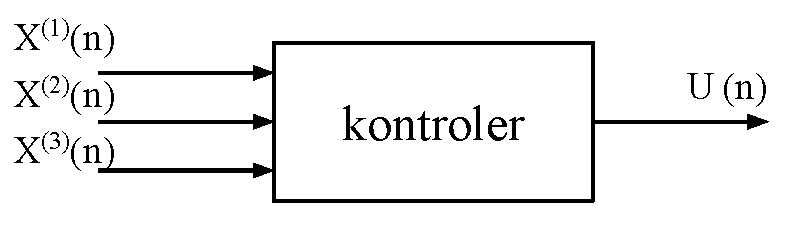
\includegraphics[width=0.5\textwidth]{images/kontroler.pdf}
    \caption{Model sterowania kontrolera}
    \label{fig:kontroler}
\end{figure}

Jak widać na rysunku \ref{fig:model} i \ref{fig:kontroler}, kontroler, do wyznaczenia sterowań sygnalizatorów wykorzystuje, stan obiektu sterowanego.

\vspace{1.5cm}
\textbf{Parametry algorytmu}
Działanie kontrolera można konfigurować przy użyciu trzech parametrów:
\vspace{0.5cm}

\begin{math} p \in <0, 1> \end{math} \textrm{ -- wpływ przewidywanego przepływu pojazdów na sterowanie}

\begin{math} q \in <0, 1> \end{math} \textrm{ -- wpływ aktualnego przepływu pojazdów na sterowanie}

\begin{math} r \in <0, 1> \end{math} \textrm{ -- wpływ aktualnych wielkości kolejek na sterowanie}

\begin{math} p + q + r = 1 \end{math}

\begin{math} t \in \mathbb{N} \textrm{ } t > 0 \end{math} \textrm{ -- długość cyklu świetlnego}

\vspace{1.5cm}
\textbf{Stałe algorytmu}
Stałe opisują niekonfigurowalne elementy kontrolowanego zespołu skrzyżowań.
\vspace{0.5cm}

\begin{math} s \in \mathbb{N} \end{math} \textrm{ -- liczba sygnalizatorów w kontrolowanym obszarze}

\begin{math} m \in \mathbb{N} \end{math} \textrm{ -- maksymalny możliwy do zmierzenia przepływ pojazdów [liczba pojazdów/godzina]}

\begin{equation}
	\begin{array}{c}
		K = \left[ k_{i} \right]_{i \in <0,s>}\\
		k_{i} \in \mathbb{N}
	\end{array}
\end{equation}

\begin{math} k_{i} \end{math} \textrm{ -- maksymalna możliwa wielkość kolejki przed i-tym sygnalizatorem [liczba pojazdów]}

\vspace{1.5cm}
\textbf{Zmienne stanu}
Stan sterowanego obszaru opisany jest trzema zmiennymi stanu:
\vspace{0.5cm}

\begin{equation}
	\begin{array}{c}
		X^{(1)} (n) = \left[ x^{(1)}_{i} (n) \right]_{i \in <0,s>}\\
		x^{(1)}_{i} (n) \in \mathbb{N}
	\end{array}
\end{equation}

\begin{math} x^{(1)}_{i} (n) \end{math} \textrm{ -- przewidywany przyszły przepływ pojazdów w kierunku i-tego sygnalizatora [liczba pojazdów/godzina]}

Przewidywany przepływ pojazdów jest wyznaczany na podstawie stanu sygnalizatorów sąsiadujacych kontrolerów.

\begin{equation}
	\begin{array}{c}
		X^{(2)} (n) = \left[ x^{(2)}_{i} (n) \right]_{i \in <0,s>}\\
		x^{(2)}_{i} (n) \in \mathbb{N}
	\end{array}
\end{equation}

\begin{math} x^{(2)}_{i} (n) \end{math} \textrm{ -- przepływ pojazdów w kierunku i-tego sygnalizatora w chwili n [liczba pojazdów/godzina]}

\begin{equation}
	\begin{array}{c}
		X^{(3)} (n) = \left[ x^{(3)}_{i} (n) \right]_{i \in <0,s>}\\
		x^{(3)}_{i} (n) \in \mathbb{N}
	\end{array}
\end{equation}

\begin{math} x^{(3)}_{i} (n) \end{math} \textrm{ -- wielkość kolejki przed i-tym sygnalizatorem w chwili n [liczba pojazdów]}

\vspace{1.5cm}
\textbf{Algorytm}

Proponowany jest poniższy algorytm wyznaczania nowego stanu sygnalizatorów.
\begin{enumerate}
	\item wyznaczenie wszystkich, zbiorów bezkolizyjnych stanów sygnalizatorów
	\item wyliczenie wag sygnalizatorów
	\item wyliczenie funkcji oceny jako sumy wag sygnalizatorów zezwalających na wjazd dla wyznaczonych wcześniej zbiorów
	\item wyznaczenie optymalnego, o najwyższej wartości funkcji oceny, stanu
\end{enumerate}

\vspace{0.5cm}
W pierwszym kroku algorytmu wyznaczane są wszystkie możliwe zbiory bezkolizyjnych stanów sygnalizatorów.
Spośród tak wyznaczonych zbiorów możliwy jest późniejszy wybór takiego który będzie w danym momencie optymalny.

\vspace{0.5cm}
Drugi krok pozwala wyznaczyć wagi zezwolnia na ruch przez każdy z sygnalizatorów, zgodnie ze wzorem \ref{eq:wagi}.

\begin{equation}
\label{eq:wagi}
	w_{i} (n) = p \cdot \frac{x^{(1)}_{i} (n)}{m} + q \cdot \frac{x^{(2)}_{i} (n)}{m} + r \cdot \frac{x^{(3)}_{i} (n)}{k_{i}}
\end{equation}

\begin{math} w_{i} (n) \end{math} \textrm{ -- waga i-tego sygnalizatora w chwili n}

\vspace{0.5cm}
W następnym kroku, wyliczone wagi są sumowane (\ref{eq:wagi_suma}) aby wyznaczyć wartość funkcji oceny dla każdego, przygotowanego w pierwszym kroku, zbioru.

\begin{equation}
\label{eq:wagi_suma}
	Q (X(n), S') = \sum\limit_{i \in S'} w_{i}
\end{equation}

\begin{math} S' \end{math} \textrm{ -- wyznaczony zbiór sygnalizatorów}

\vspace{0.5cm}
Na końcu wybierany jest stan optymalny, o najwyższej funkcji oceny.

\section{Uwzględnienie ograniczeń cyklów świetlnych}
Ograniczenie sekwencji faz cyklu świetlnego nie jest uwzględniane w działaniu powyżej zdefiniowanego algorytmum, podejmuje on jedynie decyzję o wydaniu zgody na ruch.

Za przestrzeganie tego jak i innych, czasowych, ograniczeń odpowiada dodatkowy komponent który przekazuje do obiektu sterowanego ostateczną decyzję. Zmiana sygnału powoduje utworzenie sekwencji sygnałów które nastąpią w kolejnych chwilach czasu. Uruchomienie sygnału zielonego jest opóźnione przez uwzględnienie czasów międzyzielonych. Również ograniczenia długości sygnałów żółtego i czerwono-żółtego są aplikowane na tym etapie. Wspomniany komponent odpowiada też za wymuszenie uruchomienia sygnału czerwonego, jak i zielonego, przynajmniej raz na cykl świetlny.

\section{Metody oceny skuteczności algorytmu}
Do oceny skuteczności algorytmu wykorzystać można określone na podstawie pracy Piotra Kawalca i Sylwii Sobieszuk-Durki \cite{kawalec+sobieszuk-durka} metody oceny. Są to:
\begin{itemize}
	\item średnie czasy przejazdu pojazdów na wybranych trasach
	\item średnialiczba zatrzymań pojazdów
	\item średnia prędkość pojazdów
\end{itemize}

Określone w ten sposób metody oceny można wykorzystać do porównania algorytmu z przypadkiem braku sterowania czy sterowaniem przy użyciu stałoczasowego, niezsynchronizowanego, programu sygnalizacji. Ocena wyników badań znajduje się w rozdziale \ref{chap:ocena}.